\section{Experiments}

\subsection{Experimental Setup}

\noindent\textbf{Grounding Benchmarks.}
We evaluate the grounding capabilities of our model on five challenging benchmarks: ScreenSpot-Pro~\cite{li2025screenspotpro}, ScreenSpot-v2~\cite{wu2024atlas}, OSWorld-G~\cite{wu2024atlas},MMBench-GUI-L2~\cite{wang2025mmbench} and VisualWebBench~\cite{liu2024visualwebbench_vwb}. These benchmarks assess the model's ability to accurately perceive and locate UI elements across common GUI pages with varying levels of difficulty, providing a comprehensive evaluation of fundamental visual grounding skills in graphical user interfaces.


\begin{table}[t]
\centering
\captionsetup{justification=justified, singlelinecheck=false}
\caption{Model Performance on Multiple GUI-grounding Benchmarks. 
Best results are in \textbf{bold}, second best are \underline{underlined}.}
\label{tab:gui_benchmark_performance}
\resizebox{\linewidth}{!}{
\begin{tabular}{l|ccccc}
\toprule
\textbf{Model} 
& ScreenSpot-Pro 
& ScreenSpot-v2 
& OSWorld-G 
& MMBench-GUI-L2 
& VisualWebBench \\
\midrule


OpenAI CUA & 23.4 & 87.9 & 36.4 & - & - \\
UI-TARS-1.5 & \underline{61.6} & 94.2 & - & - & - \\
SeedVL-1.5 & 60.9 & \textbf{95.2} & - & \underline{84.4} & 87.3 \\
InternVL3.5-30B-A3B-Instruct & - & 87.3 & 42.4 & - & - \\

UI-TARS-1.5-7B & 35.7 & 91.6 & 47.5 & 64.3 & - \\
UI-TARS-72B-DPO & 38.1 & 90.3 & - & 74.2 & 82.8 \\
Qwen2.5-VL-72B & 43.6 & 87.1 & - & 41.8 & - \\

GUI-Owl-7B & 54.9 & 92.8 & 55.9 & 80.5 & - \\
GUI-Owl-32B & 58.0 & 93.2 & 58.0 & 83.0 & - \\

Qwen3-VL-4B-Instruct & 59.5 & 94.0 & 58.2 & - & - \\
Qwen3-VL-8B-Instruct & 54.6 & 94.4 & 58.2 & - & - \\
Qwen3-30B-A3B-Instruct & 60.5 & 94.7 & 61.0 & 79.7 & 79.7 \\

\textbf{Step-GUI-4B} & 60.0 & 93.6 & \underline{66.9} & 84.0 & \textbf{90.7} \\
\textbf{Step-GUI-8B} & \textbf{62.6} & \underline{95.1} & \textbf{70.0} & \textbf{85.6} & \underline{89.7} \\
\bottomrule
\end{tabular}
}
\end{table}


\noindent\textbf{Computer Use.} OSWorld~\cite{xie2024osworld} provides a comprehensive evaluation suite consisting of 369 real-world tasks with detailed environment configurations and automated evaluation scripts. These tasks cover diverse desktop applications and require multi-step reasoning and interaction capabilities.

\noindent\textbf{Phone Use.} AndroidWorld~\cite{rawles2024androidworld} offers 116 tasks across 20 mobile applications within a live Android emulator environment. The benchmark includes dynamic task variations generated via randomized parameters, enabling robust evaluation of agent performance.

\noindent\textbf{AndroidDaily.} As described in Section~\ref{bmk_AndroidDaily}, AndroidDaily evaluates agent performance on commonly used Chinese applications with tasks categorized into three difficulty levels (L1-L3), providing insights into model capabilities on region-specific mobile interfaces.

\noindent\textbf{General Multimodal Benchmarks.}
We further evaluated the generalizability of our model on mainstream benchmarks across other multimodal domains which contains V*~\cite{wu2024v}, PhyX~\cite{shen2025phyx}, OmniOCR~\cite{Omniocr}, OCRBench~\cite{liu2024ocrbench}, LogicVista~\cite{xiao2024logicvista}, MMBench\_en~\cite{liu2024mmbench}, MMBench\_cn, MMStar~\cite{chen2024we},MathVista~\cite{lu2023mathvista},CharXiv~\cite{wang2024charxiv} and Simplevqa~\cite{cheng2025simplevqa}.

\noindent\textbf{Baselines.}
We compare our approach against state-of-the-art foundation models and specialized GUI agents: Claude-4-sonnet~\cite{claude4sonnet}, Claude-4.5-sonnet~\cite{claude45sonnet}, OpenAI CUA-o3 (Computer Use Agent)~\cite{openai_cua_o3}, Gemini-2.5-Computer Use~\cite{gemini2.5cu}, UI-TARS-1~\cite{qin2025ui_uitars1}, UI-TARS-2~\cite{wang2025ui_uitars2}, InternVL3.5~\cite{wang2025internvl3}, MobileRL-9B~\cite{xu2025mobilerl}, AutoGLm-9B~\cite{AutoGLM}, GLM4.6V~\cite{glm4.6v}, Qwen2.5VL~\cite{bai2025qwen2}, Qwen-OWL\&Mobile-Agent-v3 ~\cite{ye2025mobile_mobileagentv3}, Qwen3VL~\cite{Bai2025Qwen3VL}. These baselines represent diverse paradigms including general-purpose vision-language models, specialized computer-use models, and dedicated GUI automation agents.





\subsection{Main Results}

\noindent\textbf{Performance on Grounding Benchmarks.}
Table~\ref{tab:gui_benchmark_performance} presents a comprehensive comparison of our method against state-of-the-art baselines across five GUI grounding benchmarks. Our models, Step-GUI-4B and Step-GUI-8B, demonstrate consistently strong performance across diverse evaluation settings.

\textbf{ScreenSpot-Pro}. On ScreenSpot-Pro, which evaluates professional-level GUI grounding, Step-GUI-8B achieves the highest score of 62.6, outperforming UI-TARS-1.5 (61.6), SeedVL-1.5 (60.9), and Qwen3-30B-A3B (60.5). Step-GUI-4B also attains a competitive 60.0, surpassing models with significantly larger parameter counts such as Qwen2.5-VL-72B (43.6).

\textbf{ScreenSpot-v2}. On ScreenSpot-v2, Step-GUI-8B reaches 95.1, approaching the top-performing SeedVL-1.5 (95.2) and exceeding UI-TARS-1.5 (94.2).

\textbf{OSWorld-G}. For OSWorld-G, which measures grounding in realistic desktop environments, our models achieve substantial improvements: Step-GUI-8B attains 70.0 and Step-GUI-4B reaches 66.9, outperforming the next best Qwen3-30B-A3B (61.0) by a significant margin of +9.0 and +5.9 points respectively.

\textbf{MMBench-GUI-L2}. On MMBench-GUI-L2, Step-GUI-8B achieves the best result of 85.6, followed by Step-GUI-4B at 84.0, both surpassing SeedVL-1.5 (84.4) and GUI-Owl-32B (83.0). 

\textbf{VisualWebBench}. For VisualWebBench, Step-GUI-4B achieves the highest score of 90.7, exceeding SeedVL-1.5 (87.3) by +3.4 points.

These results validate the effectiveness of our multi-stage training pipeline: mid-training establishes robust visual grounding and agent-style format parsing, cold-start knowledge injection addresses task-critical gaps, and the iterative grounding-cleaning pipeline ensures high-quality supervision throughout training. Notably, our compact 4B and 8B models consistently match or outperform substantially larger models (30B--72B), demonstrating strong parameter efficiency.

\noindent\textbf{Performance on End-to-End Benchmarks.}
\begin{table*}[t]
\centering
\captionsetup{justification=justified, singlelinecheck=false}
\caption{Performance on End-to-End Environment Benchmarks. Best results are in \textbf{bold}, second best are \underline{underlined}. Note: We report both pass@1 and pass@3 metrics. Pass@3 (maximum 3 attempts per task) is used to mitigate environment instability issues including occasional CAPTCHA verification, virtual machine crashes, and other non-model-related failures, providing a more reliable evaluation of actual model capabilities.} 
\label{tab:online_env_benchmarks}
\small % 
\begin{tabular}{l|cc} 
\toprule
\textbf{Model} & OSWorld-Verified & AndroidWorld \\
\midrule
Claude-4-sonnet & 43.9 & - \\
Claude-4.5-sonnet & \textbf{61.4} & - \\
OpenAI CUA o3 & 23 & - \\
Gemini-2.5-Computer Use & - & 69.7 \\
SeedVL-1.5 & 34.1 & 62.1 \\
UI-TARS-1.5 & 42.5 & 64.2 \\
UI-TARS-2 & 47.5 & 73.3 \\
UI-TARS-1.5-7B & 27.4 & - \\
UI-TARS-72B-DPO & 24.0 & 46.6 \\
GUI-Owl-7B & 34.9 & 66.4 \\
Mobile-Agent-v3 & 37.7 & 73.3 \\
Qwen3-VL-4B-Instruct & 26.2 & 45.3 \\
Qwen3-VL-8B-Instruct & 33.9 & 47.6 \\
Qwen3-30B-A3B-Instruct & 30.3 & 54.3 \\
GLM-4.6V & 37.2 & 57.0 \\
MobileRL-9B & - & \textbf{80.2} \\
% AutoGLM-Phone-9B & 48.1 & \underline{75.8} \\
\midrule
Step-GUI-4B (Pass@1) & 31.9 & 63.9 \\
Step-GUI-8B (Pass@1) & 40.2 & 67.7 \\
\textbf{Step-GUI-4B (Pass@3)} & 40.4 & \underline{75.8} \\
\textbf{Step-GUI-8B (Pass@3)} & \underline{48.5} & \textbf{80.2} \\
\bottomrule
\end{tabular}
\vspace{-0.5em} 
\end{table*}

We evaluate our models on two challenging end-to-end environment benchmarks: OSWorld-Verified and AndroidWorld. Table~\ref{tab:online_env_benchmarks} presents a comprehensive comparison with state-of-the-art closed-source and open-source models.

\textbf{OSWorld-Verified.}~\cite{xie2024osworld} 
Due to the inherent instability of the OSWorld-Verified testing environment (including frequent VM crashes, substantial loading delays, and CAPTCHA interruptions), we employ the Pass@3 metric to mitigate failures caused by infrastructure issues rather than model limitations. 
On the OSWorld-Verified benchmark, our Step-GUI-8B achieves a score of 48.5, ranking second only to the closed-source Claude-4.5-sonnet (61.4) and significantly outperforming other competitive baselines. Notably, our model surpasses the powerful closed-source model OpenAI CUA o3 (23.0) by a substantial margin of +25.5 points, demonstrating superior reasoning and interaction capabilities in complex operating system environments. Our approach also outperforms specialized GUI understanding models such as SeedVL-1.5 (34.1), UI-TARS-1.5 (42.5), and UI-TARS-2 (47.5), as well as open-source alternatives like GUI-Owl-7B (34.9). Furthermore, compared to our baseline models Qwen3-VL-4B-Instruct (26.2) and Qwen3-VL-8B-Instruct (33.9), Step-GUI-8B achieves remarkable improvements of +22.3 and +14.6 points respectively, validating the effectiveness of our training pipeline and model design. The smaller Step-GUI-4B variant also demonstrates competitive performance with a score of 40.4, outperforming models with significantly larger parameters such as UI-TARS-1.5-7B (27.4).

\textbf{AndroidWorld.}~\cite{rawles2024androidworld} 
Given the significant stability challenges in the AndroidWorld testing environment (including unstable ADB communication, frequent Android emulator crashes, and system response delays), we employ the Pass@3 metric to exclude failures caused by infrastructure faults rather than model capability limitations. 
On the AndroidWorld benchmark, our Step-GUI-8B achieves state-of-the-art performance with a score of 80.2, tying with MobileRL-9B and establishing new performance standards for mobile GUI agents. This represents a substantial improvement over both closed-source and open-source methods. Specifically, our model outperforms UI-TARS-2 (73.3), Mobile-Agent-v3 (73.3), and the recent Gemini-2.5-Computer Use (69.7) by margins of +6.9, +6.9, and +10.5 points respectively. Compared to open-source GUI understanding models, Step-GUI-8B surpasses GUI-Owl-7B (66.4) by +13.8 points and SeedVL-1.5 (62.1) by +18.1 points. The performance gain over our baseline models is even more pronounced, with improvements of +34.9 points over Qwen3-VL-4B-Instruct (45.3) and +32.6 points over Qwen3-VL-8B-Instruct (47.6). Our smaller Step-GUI-4B variant achieves 75.8, securing the second-best performance among all tested models and outperforming all other open-source alternatives.

These results collectively demonstrate that our approach achieves exceptional performance across diverse GUI interaction scenarios, establishing new benchmarks for both desktop and mobile environments through our effective training pipeline and data construction methodology.

\begin{table*}[t]
\centering
\captionsetup{justification=justified, singlelinecheck=false}
\caption{Performance on AndroidDaily (Static) Benchmark. Best results are in \textbf{bold}, second best are \underline{underlined}.}
\label{tab:static_env_benchmarks}
\footnotesize
\setlength{\tabcolsep}{3pt} % 调小列间距
\resizebox{\textwidth}{!}{%
\begin{tabular}{l|ccccccccc}
\toprule
\textbf{Model} & CLICK & TYPE & SLIDE & AWAKE & INFO & COMPLETE & WAIT & LONG\_PRESS & AVG  \\
\midrule
GPT-4o & 12.65 & 52.41 & 31.17 & 10.84 & 0.00 & 44.85 & 5.88 & 0.00 & 17.73 \\
Claude-4.5-sonnet & 5.56 & 17.77 & \underline{50.65} & 1.33 & 0.00 & 53.48 & 21.18 & 0.00 & 10.90 \\
Gemini-2.5-Pro Thinking & 51.97 & 63.25 & 46.75 & 0.00 & 0.00 & 68.99 & 21.18 & \underline{33.33} & 43.74 \\
UI-TARS-1.5 & 84.43 & 73.49 & 48.05 & \underline{25.48} & 0.00 & 70.19 & 24.71 & \textbf{66.67} & 67.69 \\
\textbf{Step-GUI-4B} & \underline{87.11} & \underline{86.01} & 44.16 & \textbf{99.43} & \underline{52.01} & \underline{93.39} & \underline{74.12} & \textbf{66.67} & \underline{87.02} \\
\textbf{Step-GUI-8B} & \textbf{88.37} & \textbf{88.25} & \textbf{71.43} & \textbf{99.43} & \textbf{86.04} & \textbf{94.41} & \textbf{95.29} & \textbf{66.67} & \textbf{89.91} \\

\bottomrule
\end{tabular}
}
\vspace{-0.5em}
\end{table*}

\begin{table*}[t]
\centering
\captionsetup{justification=justified, singlelinecheck=false}
\caption{Performance on AndroidDaily (End-to-End) Benchmark.}
\label{tab:ad_end-to-end}

\resizebox{\textwidth}{!}{
\begin{tabular}{l
|ccc
|ccc
|ccc
|ccc
|c} 
\toprule
\multirow{2}{*}{\textbf{Model}} & 
\multicolumn{3}{c|}{\textbf{Task Type}} &
\multicolumn{3}{c|}{\textbf{Complexity}} &
\multicolumn{3}{c|}{\textbf{Ambiguity}} & 
\multirow{2}{*}{\textbf{Total}} \\ 

& Filter & Query & Analyze 
& Atomic & Comp. & Cond. 
& Low & Mid & High &  \\ 
\midrule


UI-TARS-1.5              & 57.64 & 65.97 & 36.71 
                         & 61.41 & 13.64 & 60.38 
                         & 57.05 & 54.90 & 57.89 & 56.64 \\ 


\textbf{Step-GUI-4B}   & 44.77 & 64.29 & 33.72 
                         & 54.03 & 19.61 & 42.86 
                         & 51.21 & 38.32 & 59.52 & 49.06  \\ 

\textbf{Step-GUI-8B}    & 52.50 & 63.82 & 32.95 
                         & 59.09 & 14.00 & 42.86  
                         & 54.08 & 44.55 & 61.54  & 52.50 \\ 
\bottomrule
\end{tabular}
}
\end{table*}

\noindent\textbf{Performance on AndroidDaily.}
We report evaluation results on both static action prediction and end-to-end task completion protocols.

\noindent\textit{Static Action Prediction.}
As shown in Table \ref{fig:android_daily_static}, Step-GUI-4B and Step-GUI-8B achieve state-of-the-art performance with average accuracies of 87.02\% and 89.91\% respectively, substantially outperforming all baseline models. UI-TARS-1.5 demonstrates competitive performance at 67.69\%, while general-purpose foundation models including GPT-4o (17.73\%), Claude-4.5-sonnet (10.90\%), and Gemini-2.5-Pro Thinking (43.74\%) lag significantly behind. This substantial performance gap indicates that Step-GUI and UI-TARS-1.5 possess superior domain-specific knowledge for Chinese mobile operations.

Across different action types, Step-GUI models consistently dominate. For basic interactions, both variants exceed 85\% accuracy on CLICK and TYPE actions. Notably, Step-GUI-8B achieves 71.43\% on SLIDE actions, significantly outperforming UI-TARS-1.5 (48.05\%), demonstrating better spatial reasoning for swipe gestures. For sophisticated operations including AWAKE, INFO, COMPLETE, WAIT, and LONG\_PRESS, Step-GUI models maintain strong performance with Step-GUI-8B achieving particularly high accuracy on INFO (86.04\%) and WAIT (95.29\%) actions.

\noindent\textit{End-to-End Task Completion.}
Table \ref{tab:ad_end-to-end} presents results where models interact with real applications. UI-TARS-1.5 achieves the highest success rate of 56.64\%, while Step-GUI-4B and Step-GUI-8B achieve comparable performance at 49.06\% and 52.50\% respectively. Despite UI-TARS-1.5's advantage in this setting, Step-GUI models demonstrate competitive end-to-end task completion capabilities, with Step-GUI-8B trailing by only 4.14 percentage points while significantly outperforming on static action prediction (89.91\% vs 67.69\%).

Analyzing by task type, all models perform best on Query tasks (requiring information retrieval) with success rates around 64-66\%, while Analyze tasks (demanding complex reasoning) prove most challenging with rates dropping to 33-37\%. For complexity dimensions, Atomic tasks show strong performance (54-61\%), while Composite tasks remain challenging for all models (14-20\%), indicating the difficulty of multi-step operation planning. Interestingly, examining instruction ambiguity reveals that Step-GUI-8B excels on high-ambiguity cases (61.54\%), surpassing UI-TARS-1.5 (57.89\%), demonstrating enhanced robustness in interpreting underspecified instructions, a critical capability for real-world deployment.


\begin{table*}[t]
\centering
\captionsetup{justification=justified, singlelinecheck=false}
\caption{Performance on Mainstream Multimodal Benchmarks. 
Best results are in \textbf{bold}, second best are \underline{underlined}.}
\label{tab:multimodal_benchmarks_adj_transposed}
\resizebox{\textwidth}{!}{
\begin{tabular}{l|ccccccc}
\toprule
\textbf{Benchmark} 
& \makecell{GLM-4.6V\\Flash}
& \makecell{Gemini-2.5\\flash-lite}
& \makecell{Qwen3-VL\\8B-Instruct}
& \makecell{Qwen3-VL-30B\\A3B-Instruct}
& \makecell{GPT5-nano\\minimal}
& \textbf{Step-GUI-4B} 
& \textbf{Step-GUI-8B} \\
\midrule

V*               &  -   &   -  & \underline{86.4} & \underline{86.4} & 66.5 & 79.1 & \textbf{89.0} \\
PhyX             &  -   &   -  & 28.3 & 31.1 & 24.0 & \underline{33.0} & \textbf{41.9} \\
OmniOCR          &  -   &   -  & \textbf{78.7} & 74.4 & 13.5 & 73.6 & \underline{77.1} \\
OCRBench         & 84.2 & 81.3 & \underline{89.7} & \textbf{90.8} & 70.1 & 84.6 & 88.0 \\
LogicVista       &  -   &   -  & 52.3 & \textbf{58.2} & 40.3 & 52.1 & \underline{53.7} \\
MMBench\_en      & 84.7 & 82.4 & \underline{89.9} & \textbf{90.8} & 51.6 & 87.2 & 89.1 \\
MMBench\_cn      & 85.8 &      & \underline{88.0} & \textbf{89.5} & 82.2 & 87.0 & \underline{88.0} \\
MMStar           & \textbf{72.9} & \underline{71.3} & 69.5 & 69.4 & 41.3 & 64.7 & 68.0 \\
MathVista\_{mini} & \underline{80.0} & 70.3 & 74.6 & \textbf{80.1} & 40.9 & 72.3 & 74.4 \\
CharXiv\_{DQ}     &  -   & 73.5 & 83.0 & \underline{85.5} & 64.4 & 84.1 & \textbf{86.3} \\
CharXiv\_{RQ}     &  -   & 44.6 & \underline{46.4} & \textbf{48.9} & 31.7 & 39.2 & 44.6 \\
SimpleVQA        &  -   & \underline{52.2} & 50.2 & \textbf{52.7} & 39.0 & 48.1 & 50.8 \\

\bottomrule
\end{tabular}}
\end{table*}


\noindent\textbf{Performance on General Multi-modal Benchmarks.}
To demonstrate that our model maintains strong general-purpose capabilities rather than being narrowly specialized for GUI tasks, we conduct comprehensive evaluations on mainstream multi-modal benchmarks. As shown in Table~\ref{tab:multimodal_benchmarks_adj_transposed}, \textbf{Step-GUI-8B} achieves superior or competitive performance across diverse evaluation scenarios compared to the base model Qwen3-VL-8B-Instruct and the larger Qwen3-30BA3B-Instruct.

Specifically, Step-GUI-8B achieves \textbf{89.0} on V*, surpassing both Qwen3-VL-8B-Instruct (86.4) and Qwen3-30BA3B-Instruct (86.4) by a significant margin. On OCRBench, our model scores \textbf{88.0}, outperforming Qwen3-VL-8B-Instruct (89.7) while maintaining comparable performance to Qwen3-30BA3B-Instruct (90.8). For mathematical reasoning evaluated on MathVista$_{mini}$, Step-GUI-8B achieves \textbf{74.4}, demonstrating strong reasoning capabilities that exceed the base model (74.6) while approaching the performance of the larger 30B model (80.1).
Notably, our model demonstrates consistent improvements across diverse benchmarks. Step-GUI-8B achieves \textbf{87.2} on MMBench\_en and \textbf{88.0} on MMBench\_cn for general multi-modal understanding, \textbf{68.0} on MMStar for visual reasoning, and strong performance on document understanding tasks (CharXiv$_{DQ}$: \textbf{86.3}, OmniOCR: \textbf{77.1}), indicating that GUI-oriented training does not compromise general multi-modal understanding capabilities. Furthermore, Step-GUI-4B, despite having only half the parameters, maintains competitive performance across most benchmarks, achieving \textbf{84.6} on OCRBench, which validates the effectiveness of our training approach.

These results demonstrate that our training methodology successfully enhances GUI-specific capabilities while \textit{preserving and even improving} general-purpose multi-modal understanding abilities. This characteristic is crucial for practical deployment, as it enables the model to handle diverse real-world tasks beyond GUI interaction without requiring separate specialized models.


\subsection{Detailed Analysis}


\subsubsection{Self-Evolving Training Dynamics}
\begin{figure}
    \centering
    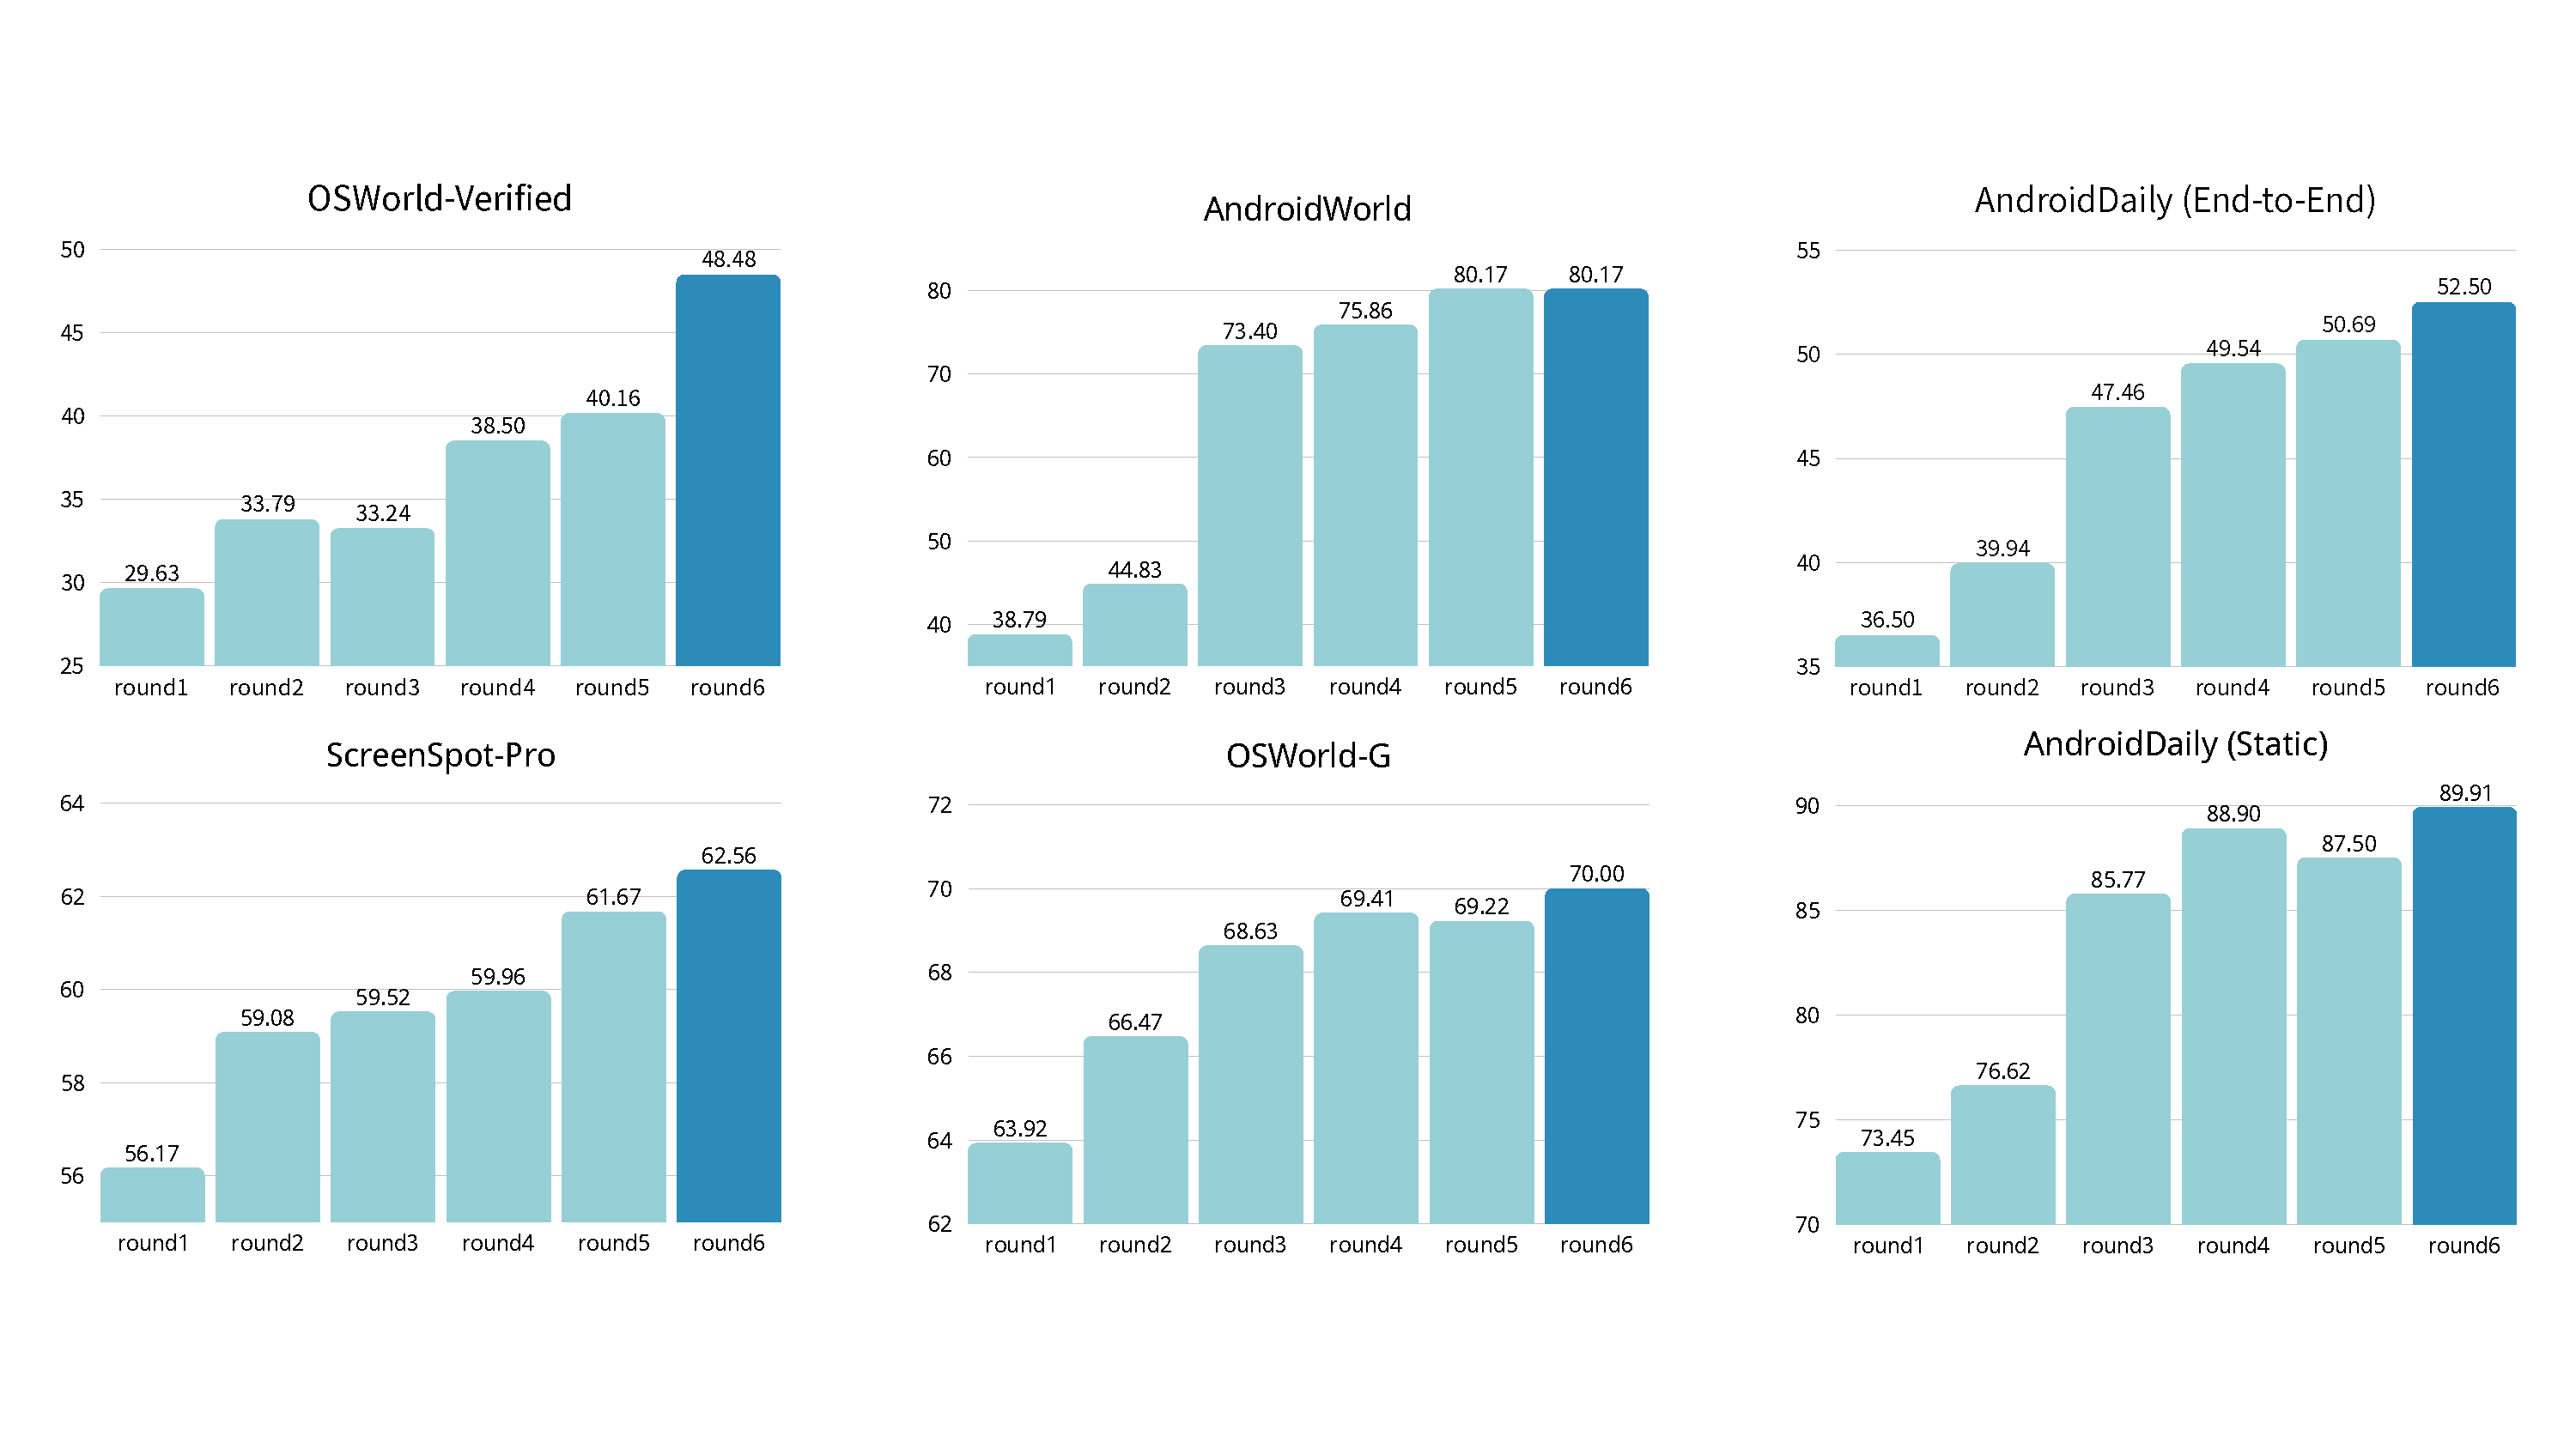
\includegraphics[width=1.0\linewidth]{figs/self-evolving.pdf}
    \caption{Performance Evolution of Step-GUI-8B Across Six Self-Evolving Training Rounds.}
    \label{fig:self_evolving}
\end{figure}


Based on the experimental data spanning Rounds 1 through 6 (as illustrated in the figure\ref{fig:self_evolving}), we validate the effectiveness of the self-evolving training framework proposed in Step-GUI. 

\noindent\textbf{"Phase Transition" on AndroidWorld.}
On the AndroidWorld benchmark, we observe a remarkable performance jump from Round 2 (44.83\%) to Round 3 (73.40\%). We attribute this surge to the Date Flow 1 (Generation) mechanism within the CSRS. 
During the initial phase (Round 1), the model addresses fundamental knowledge gaps via the Cold-Start stage. 
As the model's capabilities reach a critical threshold in Round 2, the CSRS begins to effectively capture and verify successful long-horizon trajectories generated during exploration. 
These self-discovered, high-quality trajectories enriched with Chain-of-Thought serve as high-value signals that flow back into the training pipeline, catalyzing an explosive growth in performance.

\noindent\textbf{Steady Advancement on OSWorld.}
 Compared to the mobile domain, desktop tasks on OSWorld present greater complexity. 
 Our data indicates a steady, quasi-linear improvement on OSWorld performance, rising from 29.63\% to 46.26\%. 
 This trajectory highlights the efficacy of the Date Flow 1 (Refinement). 
 By employing "Rejection Sampling" and "Self-Distillation" on challenging samples, the system continuously identifies model weaknesses near complex decision boundaries.
 It subsequently converts failed trajectories into Knowledge Data for targeted reinforcement, thereby enabling sustained breakthroughs in long-horizon, complex tasks.

Furthermore, as illustrated by the AndroidDaily (End-to-End) results in figure~\ref{fig:self_evolving}, the performance curve exhibits a smooth upward trend (49.06\% $\rightarrow$ 65.06\%). 
This stability stems from the CSRS design, which discards traditional step-level rewards in favor of rewards assigned via objective verification of final task success. 
This sparse yet high-confidence signal ensures the purity of the data fed back into the system, thereby guaranteeing robustness across multiple training iterations.
In conclusion, the synchronous capability improvements observed across diverse domains indicate that Step-GUI's self-evolving system successfully establishes a robust, general-purpose multimodal foundation through closed-loop training iterations. 
The system effectively transmutes computational resources into data quality, which subsequently evolves into model intelligence. 
This process marks a paradigm shift, transitioning the model from a reliance on human priors to a mechanism driven by self-exploration and reflection.

\begin{figure}
    \centering
    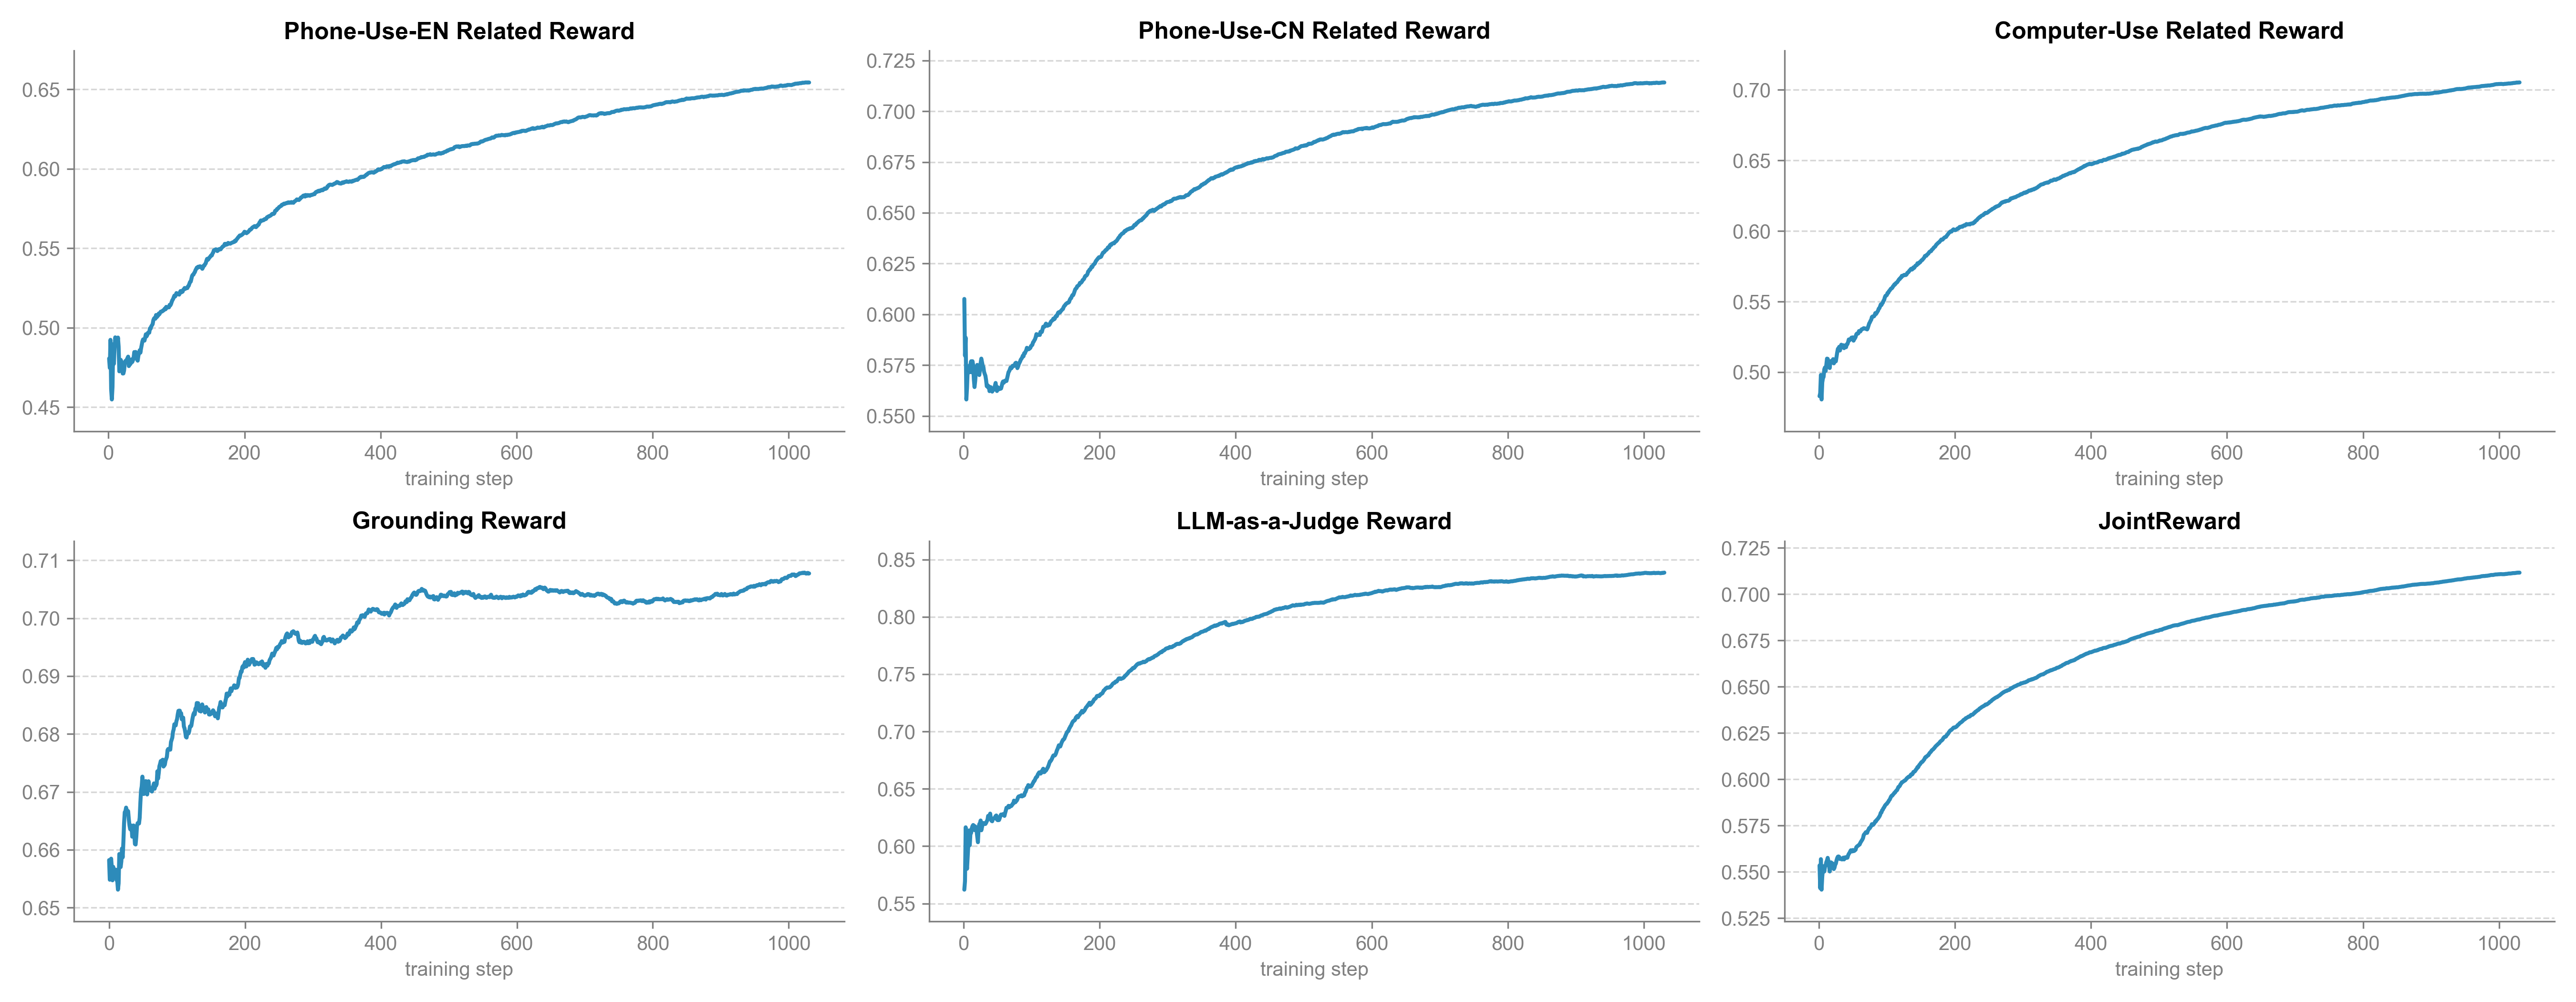
\includegraphics[width=1.0\linewidth]{figs/training_metrics_fixed_rewards.png}
    \captionsetup{justification=justified, singlelinecheck=false}
    \caption{Reward Dynamics during RLVR Training. The smooth, monotonic ascent across task-specific sub-rewards (Top) and the aggregate JointReward (Bottom Right) demonstrates stable convergence without oscillatory collapse. The strong correlation between LLM-as-a-Judge Reward and objective metrics confirms the policy improves genuine capabilities while avoiding reward hacking.}
    \label{fig:joint_reward}
\end{figure}

\subsubsection{RLVR Training: Stability and Convergence}

To rigorously assess the stability and convergence properties of the Step-GUI during RLVR stage, we monitor the optimization dynamics through a comprehensive suite of reward signals and off-policy correction metrics. 
These metrics quantify the distributional shift between the rollout policy ($\pi_{\text{rollout}}$) and the training policy ($\pi_{\text{train}}$), validating the robustness of our training.

\noindent\textbf{Reward Consistency and Alignment.}
As illustrated in Figure~\ref{fig:joint_reward}, the training process exhibits a remarkably smooth and monotonic ascent across all signal sources. The JointReward rises steadily without the oscillatory behavior or collapse often associated with RL training. 
Notably, the sub-rewards for specific capabilities, including phone-use-en, phone-use-cn, computer-use, and grounding, show high correlation with the LLM-as-a-Judge reward curve, which is demonstrated to align well with human annotations.
This synchronization confirms that our composite reward function effectively anchors the model's optimization trajectory to human-aligned reasoning, preventing reward hacking.


\begin{figure}
    \centering
    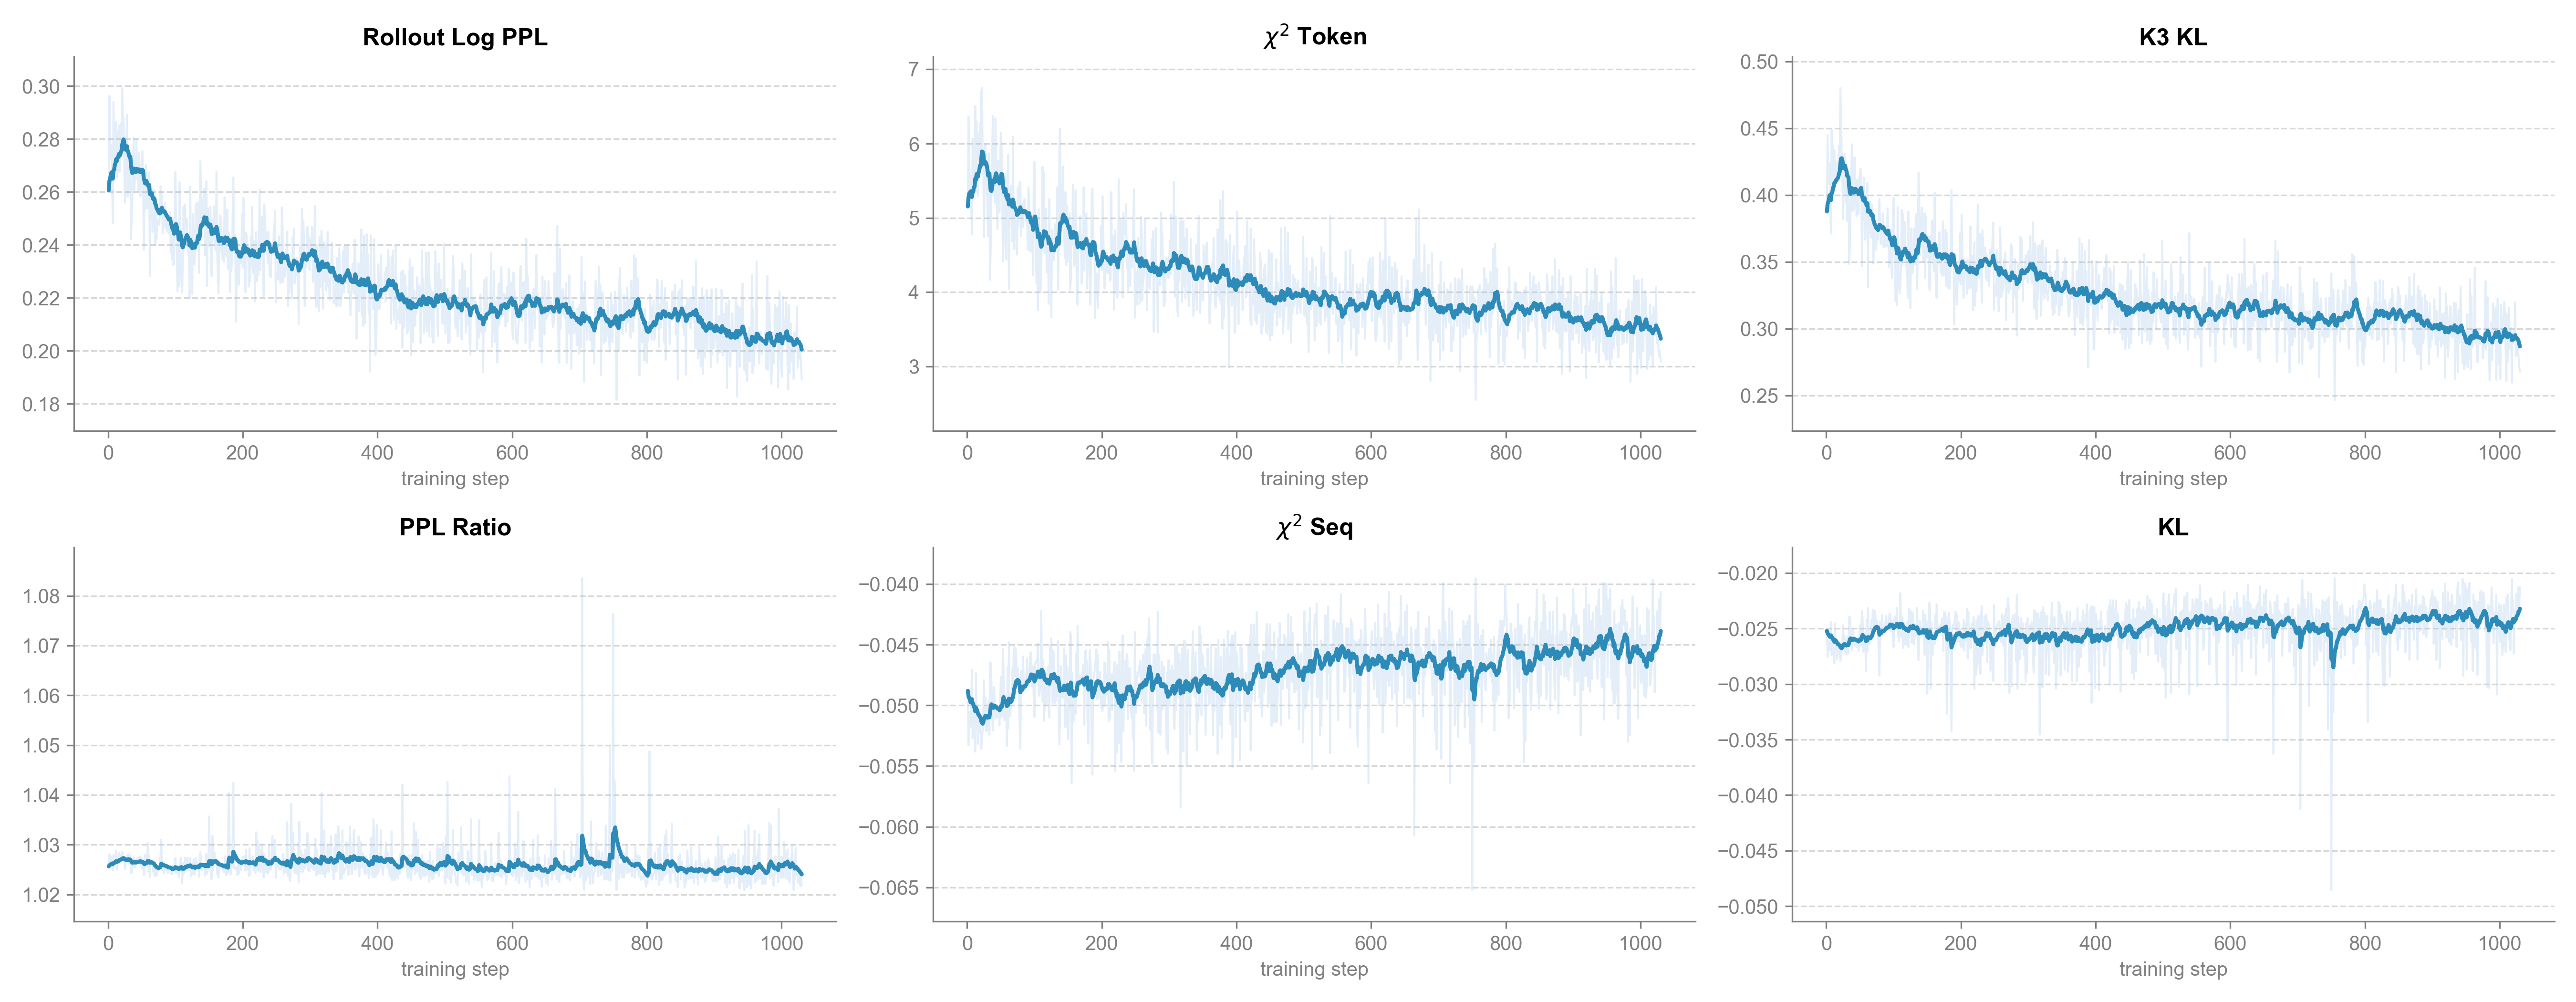
\includegraphics[width=1.0\linewidth]{figs/training_metrics_fixed_others.png}
    \captionsetup{justification=justified, singlelinecheck=false}
    \caption{Off-Policy Correction and Stability Diagnostics. The downward trends in Rollout Log PPL and $\chi^2$ (Token/Seq) variances indicate increasing model confidence and reduced gradient estimation noise. Complementing this, the decreasing K3-KL divergence demonstrates effective suppression of extreme policy deviations, while the low and stable PPL Ratio and KL confirm high synchronization between training and rollout policies, ensuring updates remain within a safe trust region.}
    \label{fig:joint_others}
\end{figure}



\noindent\textbf{Policy Synchronization.}
We scrutinize the off-policy divergence through the diagnostic metrics presented in Figure~\ref{fig:joint_others}.
First, the Rollout Log PPL displays a consistent decline (from $\sim 0.28$ to $\sim 0.20$), indicating that the rollout policy progressively gains confidence and reduces perplexity in its generated trajectories.
Concurrently, the PPL Ratio, quantifying the deviation between $\pi_{\text{train}}$ and $\pi_{\text{rollout}}$, remains consistently low and stable, fluctuating strictly between $1.02$ and $1.03$.
This dual observation confirms that even as the model becomes more deterministic, the training policy maintains high synchronization with the rollout policy, ensuring that gradient updates remain valid and effectively "on-policy" despite the inherent lag in data collection.

\noindent\textbf{Tail Risk Suppression.}
To measure distributional divergence, we monitor both standard KL divergence and the K3-KL estimator ($E[e^{\Delta} - \Delta - 1]$), which is highly sensitive to extreme deviations in the policy's tail distribution. 
While standard KL remains stable, the K3-KL metric in Figure~\ref{fig:joint_others} exhibits a distinct downward trend (from $\sim 0.45$ to $\sim 0.30$). 
This demonstrates that the model progressively minimizes "surprise" or extreme deviations from the exploration trajectory, keeping updates within a safe trust region.

\noindent\textbf{Variance Reduction.}
We further employ Importance Sampling (IS) with a sequence-truncate strategy to stabilize gradients.
The effectiveness of this mechanism is evidenced by both the token-level and sequence-level $\chi^2$ metrics, which approximate the variance of importance weights $Var(\rho)$.
As shown in Figure~\ref{fig:joint_others}, the $\chi^2$ Token metric exhibits a consistent decline from $\sim 5.5$ to $\sim 3.5$, indicating that local weight fluctuations are progressively smoothed out.
Complementing this, the $\chi^2$ Sequence maintains a stable, low-magnitude profile throughout training.
This joint behavior implies that the importance weights are becoming more uniform at both the fine-grained token level and the holistic sequence level.
Consequently, the reduction in gradient estimation noise directly substantiates the smooth convergence observed in the reward curves.

\begin{figure}
    \centering
    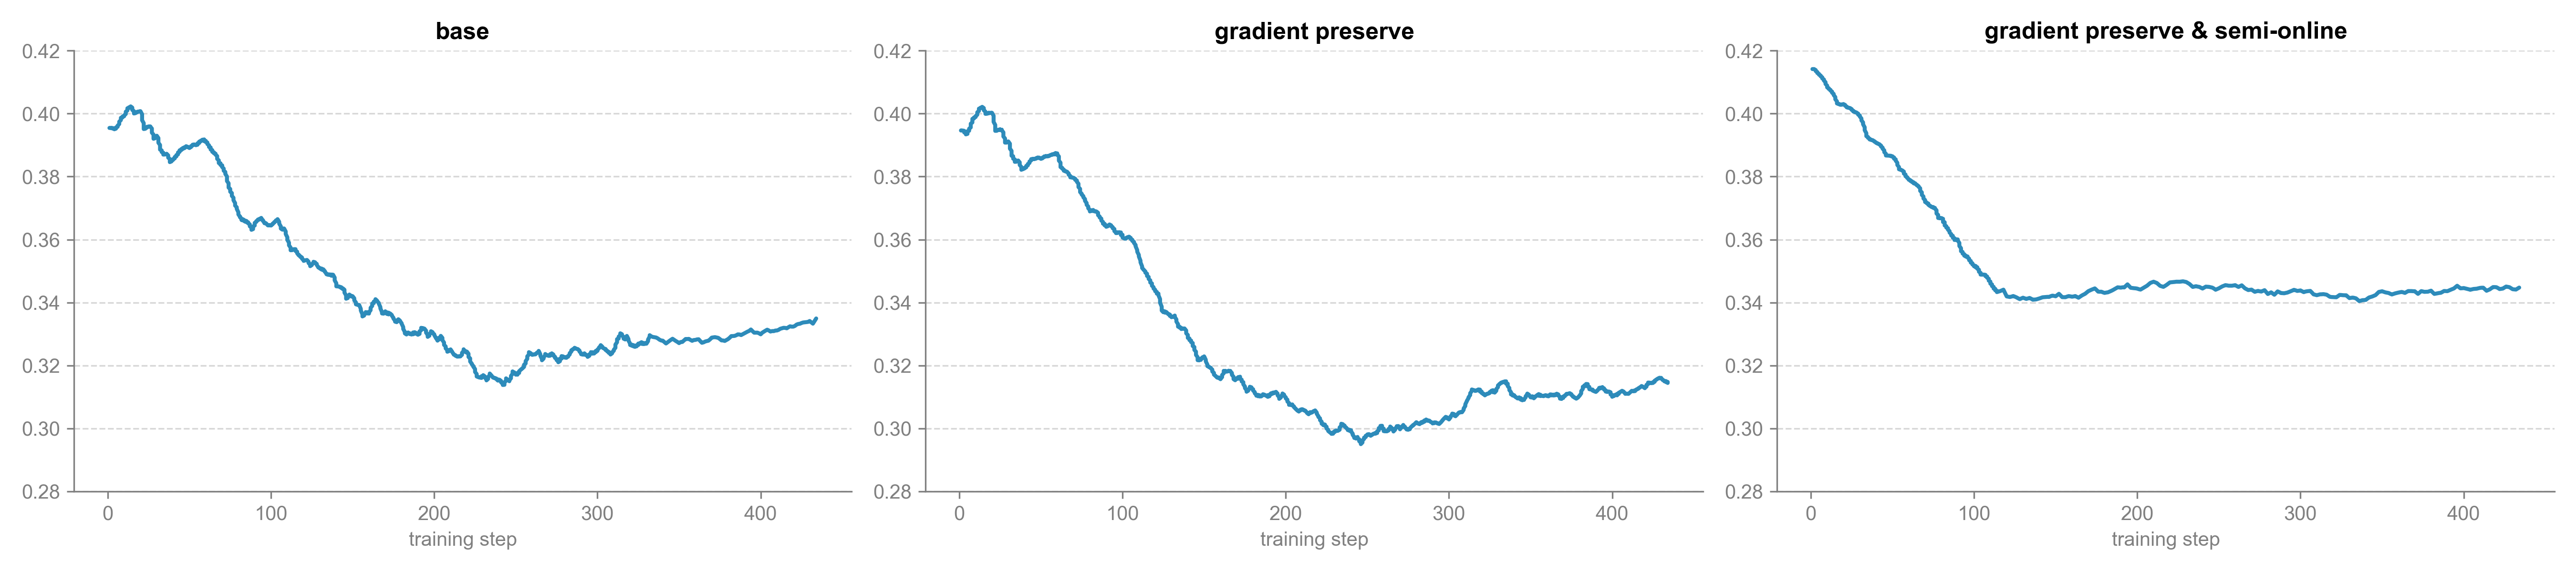
\includegraphics[width=1.0\linewidth]{figs/training_metrics_fixed_pgz.png}
    \captionsetup{justification=justified, singlelinecheck=false}
    \caption{Evolution of Policy Entropy under Different Training Strategies. Baseline GRPO (Left) shows rapid entropy decay followed by stabilization. Gradient Preservation (Middle) further reduces entropy, indicating tighter exploitation but risking mode collapse. Semi-Online strategy (Right) significantly revitalizes entropy by injecting ground-truth hints into failed rollouts, effectively disrupting narrow distributions and sustaining healthy exploration as a counter-force to premature convergence.}
    \label{fig:entropy}
\end{figure}
% pgz
\noindent\textbf{Training Entropy.}
To evaluate exploration-exploitation dynamics, we analyze policy entropy evolution in Figure~\ref{fig:entropy}. 
The baseline GRPO (Left) exhibits rapid decay followed by stabilization. 
Integrating Gradient Preservation (Middle) leads to a further reduction in entropy, indicating tighter exploitation of clipped samples but a heightened risk of mode collapse. 
In contrast, the Semi-Online strategy (Right) significantly revitalizes entropy levels. 
By injecting ground-truth hints into failed rollouts, this mechanism effectively disrupts narrow distributions and sustains healthy exploration, serving as a crucial counter-force to premature convergence.
